\documentclass[]{book}
\usepackage{lmodern}
\usepackage{amssymb,amsmath}
\usepackage{ifxetex,ifluatex}
\usepackage{fixltx2e} % provides \textsubscript
\ifnum 0\ifxetex 1\fi\ifluatex 1\fi=0 % if pdftex
  \usepackage[T1]{fontenc}
  \usepackage[utf8]{inputenc}
\else % if luatex or xelatex
  \ifxetex
    \usepackage{mathspec}
  \else
    \usepackage{fontspec}
  \fi
  \defaultfontfeatures{Ligatures=TeX,Scale=MatchLowercase}
\fi
% use upquote if available, for straight quotes in verbatim environments
\IfFileExists{upquote.sty}{\usepackage{upquote}}{}
% use microtype if available
\IfFileExists{microtype.sty}{%
\usepackage{microtype}
\UseMicrotypeSet[protrusion]{basicmath} % disable protrusion for tt fonts
}{}
\usepackage[margin=1in]{geometry}
\usepackage{hyperref}
\hypersetup{unicode=true,
            pdftitle={Modern Statistics 4 Data Science},
            pdfauthor={Joshua Loftus},
            pdfborder={0 0 0},
            breaklinks=true}
\urlstyle{same}  % don't use monospace font for urls
\usepackage{natbib}
\bibliographystyle{apalike}
\usepackage{color}
\usepackage{fancyvrb}
\newcommand{\VerbBar}{|}
\newcommand{\VERB}{\Verb[commandchars=\\\{\}]}
\DefineVerbatimEnvironment{Highlighting}{Verbatim}{commandchars=\\\{\}}
% Add ',fontsize=\small' for more characters per line
\usepackage{framed}
\definecolor{shadecolor}{RGB}{248,248,248}
\newenvironment{Shaded}{\begin{snugshade}}{\end{snugshade}}
\newcommand{\KeywordTok}[1]{\textcolor[rgb]{0.13,0.29,0.53}{\textbf{#1}}}
\newcommand{\DataTypeTok}[1]{\textcolor[rgb]{0.13,0.29,0.53}{#1}}
\newcommand{\DecValTok}[1]{\textcolor[rgb]{0.00,0.00,0.81}{#1}}
\newcommand{\BaseNTok}[1]{\textcolor[rgb]{0.00,0.00,0.81}{#1}}
\newcommand{\FloatTok}[1]{\textcolor[rgb]{0.00,0.00,0.81}{#1}}
\newcommand{\ConstantTok}[1]{\textcolor[rgb]{0.00,0.00,0.00}{#1}}
\newcommand{\CharTok}[1]{\textcolor[rgb]{0.31,0.60,0.02}{#1}}
\newcommand{\SpecialCharTok}[1]{\textcolor[rgb]{0.00,0.00,0.00}{#1}}
\newcommand{\StringTok}[1]{\textcolor[rgb]{0.31,0.60,0.02}{#1}}
\newcommand{\VerbatimStringTok}[1]{\textcolor[rgb]{0.31,0.60,0.02}{#1}}
\newcommand{\SpecialStringTok}[1]{\textcolor[rgb]{0.31,0.60,0.02}{#1}}
\newcommand{\ImportTok}[1]{#1}
\newcommand{\CommentTok}[1]{\textcolor[rgb]{0.56,0.35,0.01}{\textit{#1}}}
\newcommand{\DocumentationTok}[1]{\textcolor[rgb]{0.56,0.35,0.01}{\textbf{\textit{#1}}}}
\newcommand{\AnnotationTok}[1]{\textcolor[rgb]{0.56,0.35,0.01}{\textbf{\textit{#1}}}}
\newcommand{\CommentVarTok}[1]{\textcolor[rgb]{0.56,0.35,0.01}{\textbf{\textit{#1}}}}
\newcommand{\OtherTok}[1]{\textcolor[rgb]{0.56,0.35,0.01}{#1}}
\newcommand{\FunctionTok}[1]{\textcolor[rgb]{0.00,0.00,0.00}{#1}}
\newcommand{\VariableTok}[1]{\textcolor[rgb]{0.00,0.00,0.00}{#1}}
\newcommand{\ControlFlowTok}[1]{\textcolor[rgb]{0.13,0.29,0.53}{\textbf{#1}}}
\newcommand{\OperatorTok}[1]{\textcolor[rgb]{0.81,0.36,0.00}{\textbf{#1}}}
\newcommand{\BuiltInTok}[1]{#1}
\newcommand{\ExtensionTok}[1]{#1}
\newcommand{\PreprocessorTok}[1]{\textcolor[rgb]{0.56,0.35,0.01}{\textit{#1}}}
\newcommand{\AttributeTok}[1]{\textcolor[rgb]{0.77,0.63,0.00}{#1}}
\newcommand{\RegionMarkerTok}[1]{#1}
\newcommand{\InformationTok}[1]{\textcolor[rgb]{0.56,0.35,0.01}{\textbf{\textit{#1}}}}
\newcommand{\WarningTok}[1]{\textcolor[rgb]{0.56,0.35,0.01}{\textbf{\textit{#1}}}}
\newcommand{\AlertTok}[1]{\textcolor[rgb]{0.94,0.16,0.16}{#1}}
\newcommand{\ErrorTok}[1]{\textcolor[rgb]{0.64,0.00,0.00}{\textbf{#1}}}
\newcommand{\NormalTok}[1]{#1}
\usepackage{longtable,booktabs}
\usepackage{graphicx,grffile}
\makeatletter
\def\maxwidth{\ifdim\Gin@nat@width>\linewidth\linewidth\else\Gin@nat@width\fi}
\def\maxheight{\ifdim\Gin@nat@height>\textheight\textheight\else\Gin@nat@height\fi}
\makeatother
% Scale images if necessary, so that they will not overflow the page
% margins by default, and it is still possible to overwrite the defaults
% using explicit options in \includegraphics[width, height, ...]{}
\setkeys{Gin}{width=\maxwidth,height=\maxheight,keepaspectratio}
\IfFileExists{parskip.sty}{%
\usepackage{parskip}
}{% else
\setlength{\parindent}{0pt}
\setlength{\parskip}{6pt plus 2pt minus 1pt}
}
\setlength{\emergencystretch}{3em}  % prevent overfull lines
\providecommand{\tightlist}{%
  \setlength{\itemsep}{0pt}\setlength{\parskip}{0pt}}
\setcounter{secnumdepth}{5}
% Redefines (sub)paragraphs to behave more like sections
\ifx\paragraph\undefined\else
\let\oldparagraph\paragraph
\renewcommand{\paragraph}[1]{\oldparagraph{#1}\mbox{}}
\fi
\ifx\subparagraph\undefined\else
\let\oldsubparagraph\subparagraph
\renewcommand{\subparagraph}[1]{\oldsubparagraph{#1}\mbox{}}
\fi

%%% Use protect on footnotes to avoid problems with footnotes in titles
\let\rmarkdownfootnote\footnote%
\def\footnote{\protect\rmarkdownfootnote}

%%% Change title format to be more compact
\usepackage{titling}

% Create subtitle command for use in maketitle
\newcommand{\subtitle}[1]{
  \posttitle{
    \begin{center}\large#1\end{center}
    }
}

\setlength{\droptitle}{-2em}
  \title{Modern Statistics 4 Data Science}
  \pretitle{\vspace{\droptitle}\centering\huge}
  \posttitle{\par}
  \author{Joshua Loftus}
  \preauthor{\centering\large\emph}
  \postauthor{\par}
  \predate{\centering\large\emph}
  \postdate{\par}
  \date{2019-12-06}

\usepackage{booktabs}

\usepackage{amsthm}
\newtheorem{theorem}{Theorem}[chapter]
\newtheorem{lemma}{Lemma}[chapter]
\theoremstyle{definition}
\newtheorem{definition}{Definition}[chapter]
\newtheorem{corollary}{Corollary}[chapter]
\newtheorem{proposition}{Proposition}[chapter]
\theoremstyle{definition}
\newtheorem{example}{Example}[chapter]
\theoremstyle{definition}
\newtheorem{exercise}{Exercise}[chapter]
\theoremstyle{remark}
\newtheorem*{remark}{Remark}
\newtheorem*{solution}{Solution}
\begin{document}
\maketitle

{
\setcounter{tocdepth}{1}
\tableofcontents
}
\chapter{Outline}\label{outline}

This course surveys theory and methods addressing important statistical
aspects of data science with a focus on high-dimensional data,
statistical learning, and causal inference. We will begin with advances
in hypothesis testing such as control of the false discovery rate for
multiple comparisons. Then we will discuss statistical theory for
popular learning and model selection methods such as the lasso,
including recent advances in post-selection inference. Finally, after
reviewing frameworks for causal inference the course will conclude by
reading literature on the application of statistical learning methods to
causal inference. Throughout the course we will combine theory, through
mathematical understanding, with practice, through empirical
understanding and competency with applications such as simulation
studies. We assume a working knowledge of probability and linear
algebra, familiarity with statistics, and willingness to code in the R
statistical programming language, but otherwise the course is
self-contained.

Topics:

\begin{itemize}
\tightlist
\item
  Ethical data science
\item
  Foundations of statistical inference
\item
  Large-scale hypothesis testing
\item
  Inference for causal effects
\item
  Foundations of regression models
\item
  Machine learning and high-dimensional regression
\item
  Adjusting inference for model selection
\item
  Machine learning in causal inference
\end{itemize}

Textbooks:

Selected readings from the following references (subject to minor
changes), all of which have free PDFs available by following these
links.

\begin{itemize}
\tightlist
\item
  \href{http://web.stanford.edu/~hastie/CASI/}{Computer Age Statistical
  Inference: Algorithms, Evidence and Data Science} by Bradley Efron and
  Trevor Hastie
\item
  \href{https://web.stanford.edu/~hastie/StatLearnSparsity/}{Statistical
  Learning with Sparsity: The Lasso and Generalizations} by Trevor
  Hastie, Robert Tibshirani, and Martin Wainwright
\item
  \href{https://www.hsph.harvard.edu/miguel-hernan/causal-inference-book/}{Causal
  Inference} by Miguel Hernán and Jamie Robins
\item
  \href{https://mitpress.mit.edu/books/elements-causal-inference}{Elements
  of Causal Inference: Foundations and Learning Algorithms} by Jonas
  Peters, Dominik Janzing and Bernhard Schölkopf
\end{itemize}

\chapter{Introduction}\label{intro}

This section will contain a few motivating examples illustrating
problems like

\begin{itemize}
\tightlist
\item
  Association vs causation
\item
  Regression model selection
\item
  Multiple testing and p-hacking
\item
  Fair algorithms
\item
  Dangers of AI
\end{itemize}

\chapter{Ethical data science}\label{ethical-data-science}

Data and information technology are powerful tools that can be used for
good or evil. As with other human technologies (e.g.~fossil fuel energy,
nuclear technology) \textbf{the consequences of data science will depend
on who uses it and for what purposes}. Much of humanity now relies on
information technology in almost all aspects of our lives, and many data
scientists are doing work that becomes part of this infrastructure. Like
city planners, our decisions can have major impacts on everyone.

Data science can be directly harmful in ways that are easy to
anticipate, but it can also do damage in ways that are subtle and more
difficult to predict. The great diversity of people who may be affected
by our work can make it challenging to anticipate all the potential
harms, but making a thorough effort to do so is part of the
responsibility of an ethical data scientist. Even if we are not
particularly altruistic, we should also remember that blame for ethical
failures typically does not fall on machines, but on the people who
built or used them. For this reason it can be in our own best interests
to avoid doing the kind of data science that brings about harm.

``\href{https://en.wikipedia.org/wiki/Primum_non_nocere}{First, do no
harm}'' is a phrase associated with medical ethics, and it's clearly
relevant to data science as well. But as the phrase itself indicates,
\textbf{avoiding harm is only the beginning}. A broader conception of
ethics could include concern for freedom from the influence of
data-driven decisions based on factors outside our control. Data science
should be transparent and reproducible, qualities which are also
desirable from the standpoint of scientific methodology. And statistical
methods can only help us make sense of uncertainty if we use them in a
principled and ethical fashion, otherwise we can end up deceiving
ourselves and others.

The goal of this section (as with the rest of the book) is not to
provide a list of principles or rules to memorize, but to motivate you
to cultivate your own judgment and provide some starting points to help
begin that process. Technology enables progress, but whether it is a
software library for deep neural networks or something as simple as an
abacus it can also encourage action without intention, decision without
reflection. Your own internal sense of ethics may be our last line of
defense in the basic human struggle for autonomy within the rapidly
changing sociotechnical constraints of modernity. Your principled use of
data science may be necessary to safeguard the epistemic autonomy of
science from the financial pressures of the information economy.

\section{Motivating example: fair
algorithms}\label{motivating-example-fair-algorithms}

There are many types of tasks in data science for which ethics is
relevant, but we will continue focusing mainly on supervised learning.
Suppose that we have data \((Y, X, A)\) where \(Y\) is an \emph{outcome
variable}, \(A\) is a \emph{sensitive attribute} (e.g.~racial and/or
gender identity), and \(X\) the remaining \emph{predictors} which are
considered nominally non-sensitive. We are tasked with learning a
function to predict \(Y\), that is we hope that \[
Y \approx f(X, A) \quad \text{or (more realistically)} \quad E[Y|X, A] \approx f(X, A)
\] for some function \(f\) which we can estimate from a set of training
data. However, since \(A\) is a sensitive attribute, we would also like
for the predictions from our learned function to ``not depend'' on \(A\)
in some sense. For example, we might consider functional independence:
\[
\hat Y = \hat f(X)
\] where the function does not take \(A\) as an explicit input. We'll
come back to this later, but for now let's consider a few concrete
examples of such a task to understand why we might want the predictions
to ``not depend'' on \(A\).

\begin{itemize}
\tightlist
\item
  Employment (ads): \(Y\) is a score used to determine whether or not to
  interview or hire a candidate (or serve an ad for the position), \(X\)
  some covariates like educational status and years of experience, and
  \(A\) age or an indicator of whether someone is at least 40 years old.
  In the US,
  \href{https://en.wikipedia.org/wiki/Age_Discrimination_in_Employment_Act_of_1967}{it
  is illegal} to discriminate in employment on the basis of age for
  people age 40 and above.
\item
  Insurance/lending: \(Y\) is a risk score used to price an insurance
  policy or loan decision, \(X\) some covariates about employment status
  and financial credit history, and \(A\) could be racial and/or gender
  identity. In 2019, Apple--one of the largest companies in the world
  and a veteran of the tech industry which employs many data
  scientists--released a credit card and caused an immediate scandal
  when people noticed that spending limits were drastically different
  between men and women, even for the
  \href{https://www.wired.com/story/the-apple-card-didnt-see-genderand-thats-the-problem/}{co-founder
  of Apple} and his spouse.
\item
  Criminal arrests: \(Y\) indicates an outcome like arrest, the \(X\)
  covariates might record past arrest history and age, and \(A\) could
  be racial or religious identity. One underlying concern is that people
  are targeted by law enforcement differentially, resulting in different
  rates of arrest even if the underlying rates of criminal activity are
  not different.
\end{itemize}

This list is not comprehensive and only meant to give some indication of
the kinds of problems that might arise in fair algorithms. In each
example, the past data \((Y, X, A)\) is used to learn a function
\(\hat f\) which predicts future outcomes from the covariates, and these
predictions will be used to make decisions that affect people. But the
past data may encode patterns due to historical injustices.

\subsection{A brief historical
interlude}\label{a-brief-historical-interlude}

Let's consider the insurance/lending example and the history of
oppression and violence in the United States toward African-Americans.
Economic changes occur slowly, if at all, at the time scale of
generations. The graphs below, created under the supervision of
\href{https://en.wikipedia.org/wiki/W._E._B._Du_Bois}{W. E. B. Du Bois}
for
\href{https://www.smithsonianmag.com/history/first-time-together-and-color-book-displays-web-du-bois-visionary-infographics-180970826/}{exhibition}
at the 1900 Exposition Universelle in Paris, show that after the end of
centuries of slavery the accumulation of wealth among African Americans
in the state of Georgia happened gradually, over decades, and was met
with resistance.

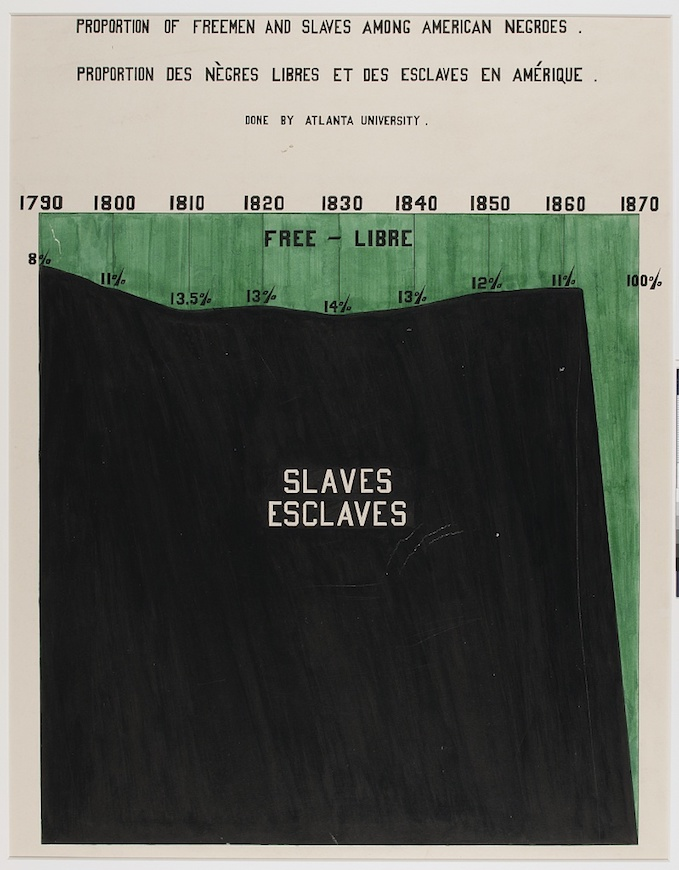
\includegraphics{dubois1.jpg} 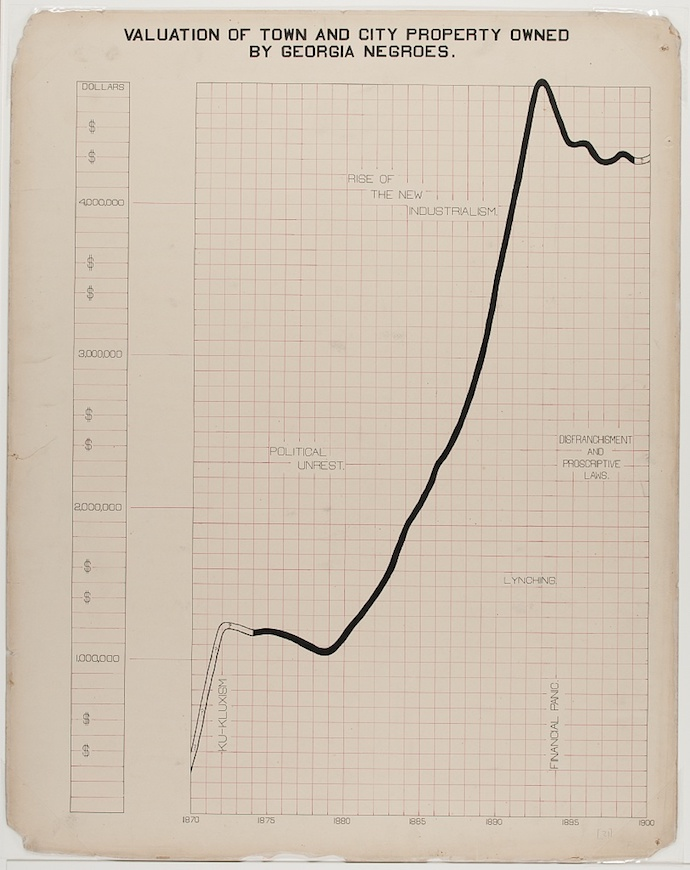
\includegraphics{dubois2.jpg}

Before the 1960's civil rights movement, racist
``\href{https://en.wikipedia.org/wiki/Jim_Crow_laws}{Jim Crow}'' laws
continued to be obstacles to black Americans, and mass violence
including riots resulted in deaths, destruction, and further setbacks.
In one of the more extreme examples of this, in 1921 the wealthiest
black community in the US (known as
``\href{https://en.wikipedia.org/wiki/Tulsa_race_riot}{Black Wall
Street}'') was attacked by thousands of white Americans who destroyed 35
blocks of homes, including with bombs dropped from airplanes, left about
10,000 black Americans homeless and killed on the order of a hundred
people.

It's not easy to find data on median family wealth by race going back
before the 1980's, but a
\href{https://www.minneapolisfed.org/research/institute-working-papers/income-and-wealth-inequality-in-america-1949-2016}{recent
paper} estimated this going back to almost 1950 and the result is
\href{https://qz.com/1368251/black-income-is-half-that-of-white-households-just-like-it-was-in-the-1950s/}{stark}:

\begin{figure}
\centering
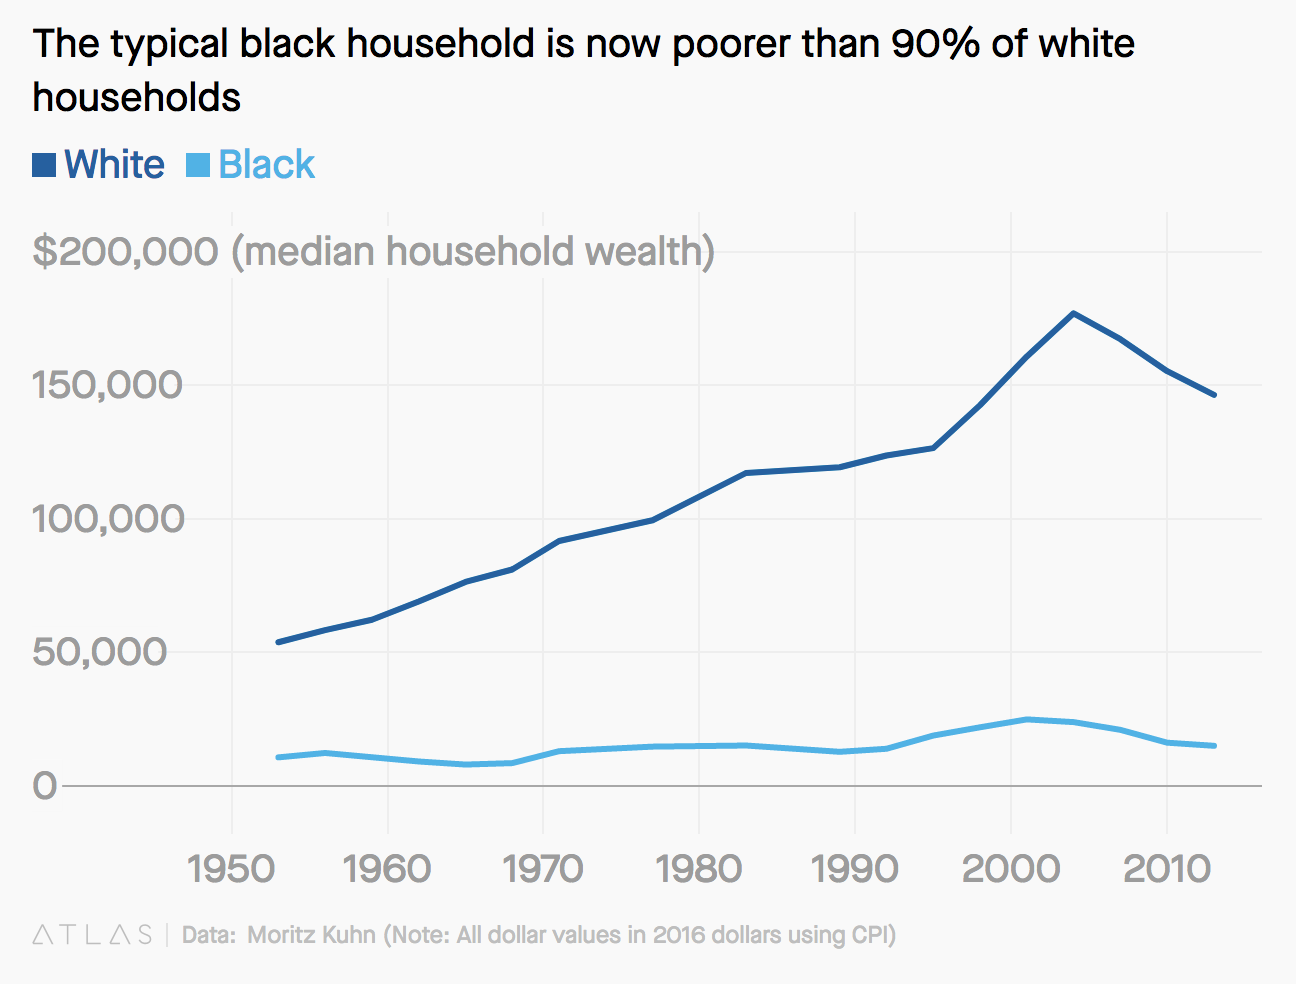
\includegraphics{medianwealth.png}
\caption{}
\end{figure}

Median family wealth for black families has remained low from the
pre-civil rights era through to the present. This brief and very high
level historical summary gives an idea of the context that our
``training data'' for a risk assessment algorithm comes from. There are
many important details we have skipped, including the practices of
``\href{https://en.wikipedia.org/wiki/Redlining}{redlining}'' and
``\href{https://uncpress.org/book/9781469653662/race-for-profit/}{predatory}
\href{https://www.nbcnews.com/think/opinion/undermining-black-homeownership-keeanga-yamahtta-taylor-podcast-transcript-ncna1063426}{inclusion}.''

Switching to briefly consider the example of gender and employment,
there has also been a slow and historically recent change in the
fundamental relationships and conditions that generate the training
data. Consider the labor force participation of women in the United
States from about 1950 to the present:

\begin{figure}
\centering
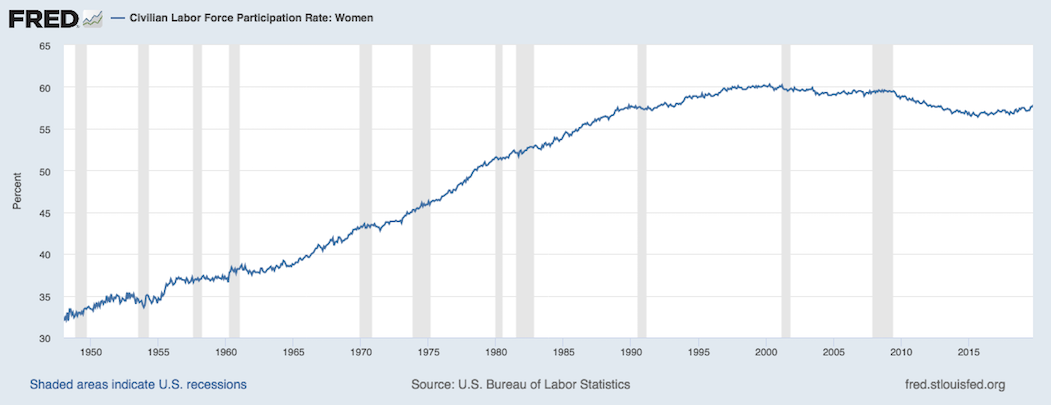
\includegraphics{fredfemalelabor.png}
\caption{}
\end{figure}

Or, even more closely related to data science, consider the
\href{https://www.npr.org/sections/money/2014/10/21/357629765/when-women-stopped-coding}{percent
of degrees} awarded to women in computer science in comparison to some
other fields:

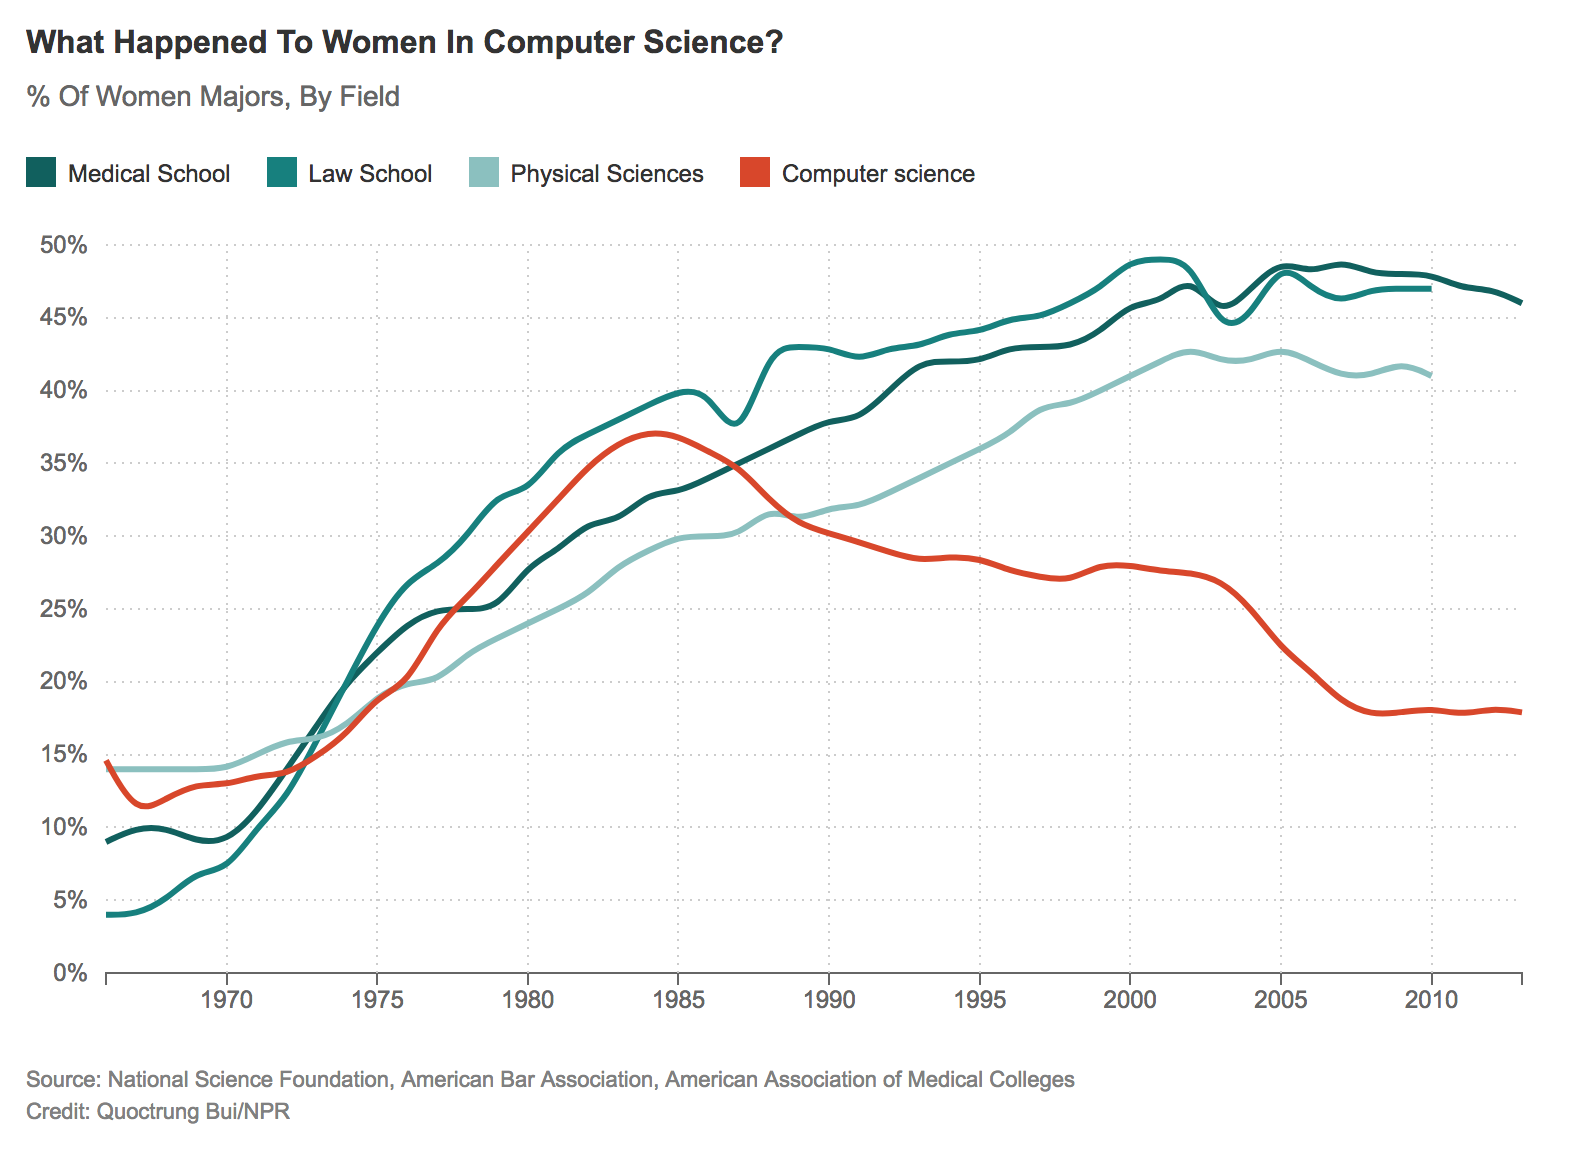
\includegraphics{womenincs.png} (Statistics does a little bit better
than computer science in this regard).

Notice that I am appealing to empirical facts and data to make the case
that some sort of adjustment may be necessary to make fair algorithms
using training data from an unfair past. Do these facts seem relevant?
What kinds of adjustments would be acceptable or desirable? How do we
know what's fair or unfair to begin with? We'll now consider some
principles and frameworks to help us answer questions like these, moving
from the general to the more specific as we progress.

\emph{Discussion}:

\begin{itemize}
\tightlist
\item
  Do you know of other examples like these where historical injustices
  can result in data showing poor outcomes for a particular group of
  people?
\item
  Where do systems of
  \href{https://en.wikipedia.org/wiki/Historical_race_concepts}{racial
  categorization} come from, and how have they
  \href{https://www.pewsocialtrends.org/interactives/multiracial-timeline/}{changed
  over time}?
\item
  Where does
  \href{https://en.wikipedia.org/wiki/Social_construction_of_gender}{gender
  identity} come from, and is there any reason to
  \href{https://chance.amstat.org/2014/11/visiphilia/}{(dis)believe}
  gender inherently relates to ability in computing or mathematics?
\end{itemize}

\begin{quote}
The double-edged sword of data shows just how important it is to
understand how structures of power and privilege operate in the world.
The questions we might ask about these structures can relate to issues
of gender in the workplace, {[}\ldots{}{]}. Or they can relate to issues
of broader social inequality, {[}\ldots{}{]}. So one thing you will
notice throughout this book is that not all of our examples are about
women--and deliberately so. This is because data feminism is about more
than women. It's is about more than gender. Put simply: Data Feminism is
a book about power in data science. Because feminism, ultimately, is
about power too. It is about who has power and who doesn't, about the
consequences of those power differentials, and how those power
differentials can be challenged and changed.
\end{quote}

From \href{https://bookbook.pubpub.org/pub/dgv16l22}{Data Feminism} by
Catherine D'Ignazio and Lauren Klein

\section{Philosophy of ethics}\label{philosophy-of-ethics}

\subsection{Meta-ethics}\label{meta-ethics}

Meta-ethics is about high level questions like:

\begin{itemize}
\tightlist
\item
  Can moral statements be factual, or are they just expressions of
  taste/preference?
\item
  Are morals universal, relative, or meaningless?
\item
  What approaches can be used to establish moral claims? Can we rely on
  intuition, reason, empirical evidence?
\end{itemize}

Although these are fascinating questions we will not dwell on them.
We'll proceed under a working assumption that (1) moral claims are
meaningful (and important) enough to merit our careful study, and (2)
the above methods for establishing them are all valid enough to use but
also imperfect and subject to error. We can also remember to reconsider
these questions in light of the concepts and examples we focus on below.

\subsection{Normative ethics}\label{normative-ethics}

There are a variety of qualitatively different theoretical approaches
for how we can determine what is ethical or moral. These approaches are
not mutually exclusive or exhaustive, so we do not have to choose one of
them or limit our thinking to using only these ideas.

\subsubsection{Consequentialist ethics}\label{consequentialist-ethics}

Consequentialism judges actions based on effects caused by those acts.
One common form of this is \textbf{utilitarianism}: to choose actions
resulting in the greatest good for the greatest number of people. There
are difficulties in defining utility, trading off between different
people, deciding whether to judge specific acts or general rules for
guiding actions, and uncertainty about predicting consequences. The last
issue, predicting consequences, is one where the intersection with data
science is particularly relevant.

\subsubsection{Deontological ethics}\label{deontological-ethics}

Deontology judges actions without necessarily referencing the effects
caused by these actions. Actions can be considered good even if they
result in bad consequences as long as they adhere to moral rules.
Provided we understand which rules we have a duty to follow this may be
simpler than consequentialism because we may not need to predict the
consequences of our actions. However, if there is no room to override
rules under special circumstances we may be obligated to suffer
extremely bad consequences.

\subsubsection{Virtue ethics}\label{virtue-ethics}

Virtue ethics judges traits, or character. A person can be moral even if
they act against deontological rules and their action causes negative
consequences, provided the person acts in accordance with a virtuous
trait. Upholding virtues is considered a good in itself, and some
virtues emphasize the social aspects of being morally good. With a
multiplicity of virtues rather than one sense of good we may have better
explanatory power, but conflicts can arise between virtues and we may
not agree on which character traits should be considered virtuous.

\emph{Discussion}:

\begin{itemize}
\tightlist
\item
  Data science is usually framed (perhaps implicitly) as utilitarian
  because of its focus on prediction/causation (consequences) and
  optimization (utility). Discuss some prototypical data science
  problems with explicitly utilitarian language, and indicate how
  non-consequentialist theories can also apply to these problems.
\item
  Deontology seems to most obviously relate to ``equal treatment''
  notions of fairness, but (1) can other fairness notions be justified
  on a deontological basis, (2) how would other ethical theories
  justify/criticize equal treatment?
\item
  How do we know/decide which things are virtuous? Is intelligence a
  virtue? How/when can we decide between contradicting virtues?
\item
  For each of the previous normative frameworks, use that framework to
  describe an argument (1) supporting the practice of following laws,
  and (2) supporting the practice of law-breaking under certain
  circumstances, and describe sufficient properties of those
  circumstances.
\end{itemize}

\section{Applied ethics}\label{applied-ethics}

Applied ethics in data science is the most relevant part of this topic
to our course. Normative ethical theories can be valuable for high level
reasoning, but may be too general to figure out what is good in a
specific real world scenario. To address this practical problem,
professionals in fields like biomedical ethics have developed principles
that may also be broadly applicable in data science.

\subsection{Belmont-Menlo principles}\label{belmont-menlo-principles}

Starting in 1932 the United States Public Health Service carried out a
study--the
\href{https://en.wikipedia.org/wiki/Tuskegee_syphilis_experiment}{Tuskegee
syphilis experiment}--that recruited African American men in the state
of Alabama by telling them that they would receive free healthcare. Most
of the men in the study had a disease, syphilis, but were never told by
the researchers that they had the disease, and were also never told that
they were not actually being treated. By 1947 it was well known that the
drug penicillin was an effective treatment, but the study participants
were prevented from receiving this treatment. Other researchers who knew
of the study raised objections, including one doctor who wrote to the
study authors in 1965 but was ignored. The US Centers for Disease
Control intended to continue the study until all participants had died.
In 1968
\href{https://www.nature.com/articles/d41586-019-00900-9}{William Carter
Jenkins}, an African American statistician, founded and wrote a
newsletter where he also tried to raise awareness of the experiment.
Another whistleblower came forward in 1972 and finally some major
newspapers picked up the story and the study was ended. By that time
some of the men had died of syphilis or related complications, some of
their wives had become infected, and some of their children were born
with syphilis. Jenkins produced \href{https://youtu.be/3e5VfgsGp1k}{a
documentary} interviewing survivors of the experiment in 2002 when some
of them were still alive.

Under national attention the study became a scandal, and in response the
government formed a National Commission for the Protection of Human
Subjects of Biomedical and Behavioral Research. The Commission spent
several years authoring a report, commonly referred to as the
\href{https://en.wikipedia.org/wiki/Belmont_Report}{Belmont Report},
which established 3 of the 4 principles listed below. This report still
guides the Institutional Review Boards (IRB) that oversee compliance
with ethical research practices in many universities.

These principles were adapted and supplemented by the US Department of
Homeland Security Science and Technology Directorate into a
cybersecurity setting. Their
\href{https://www.dhs.gov/sites/default/files/publications/CSD-MenloPrinciplesCORE-20120803_1.pdf}{Menlo
Report} was published in 2012 and describes the four principles which
are copied verbatim below:

\subsubsection{Respect for persons}\label{respect-for-persons}

\begin{quote}
Participation as a research subject is voluntary, and follows from
informed consent; Treat individuals as autonomous agents and respect
their right to determine their own best interests; Respect individuals
who are not targets of research yet are impacted; Individuals with
diminished autonomy, who are incapable of deciding for themselves, are
entitled to protection.
\end{quote}

\subsubsection{Beneficience}\label{beneficience}

\begin{quote}
Do not harm; Maximize probable benefits and minimize probable harms;
Systematically assess both risk of harm and benefit.
\end{quote}

\subsubsection{Justice}\label{justice}

\begin{quote}
Each person deserves equal consideration in how to be treated, and the
benefits of research should be fairly distributed according to
individual need, effort, societal contribution, and merit; Selection of
subjects should be fair, and burdens should be allocated equitably
across impacted subjects.
\end{quote}

\subsubsection{Respect for law and the public
interest}\label{respect-for-law-and-the-public-interest}

\begin{quote}
Engage in legal due diligence; Be transparent in methods and results; Be
accountable for actions.
\end{quote}

\subsection{The five Cs framework}\label{the-five-cs-framework}

In the book Ethics in Data Science by Mike Loukides, Hilary Mason, and
DJ Patil, the authors outline a practical framework they call the
\href{https://resources.oreilly.com/examples/0636920203964/blob/master/the_five_cs.md}{five
Cs} which we now summarize.

\subsubsection{Consent}\label{consent}

We should not collect data from people who have not explicitly agreed to
allow that data collection. Informed consent is also part of the Belmont
principle of respect for persons. To be informed means that people know
what data will be collected and what purposes it may be used for, and
can reasonably understand the consequences of their agreement to allow
data collection. Obtaining informed consent is practically mandatory for
medical research, but sadly it remains an uncommon standard regarding
data collection. There are many companies that collect data about people
without even asking.

\subsubsection{Clarity}\label{clarity}

To give informed consent someone must understand what their consent
allows. But user agreements are often hard to understand, even for
relatively well informed people, and the consequences of allowing data
collection are far from well understood by most of the people checking
the ``I agree'' box in order to continue.

\subsubsection{Consistency and trust}\label{consistency-and-trust}

Being consistent helps people set their expectations and decide whether
to trust our work. Many of the examples where data science has resulted
in undesirable outcomes generating a lot of controversy happened because
people encountered some behavior or outcome inconsistent with their
expectations.

\subsubsection{Control and transparency}\label{control-and-transparency}

After giving informed consent for their data to be collected, users
should still have control. This requires ongoing transparency about the
status of their data, and should allow users to opt in or out of
specific uses if they choose to do so even after initially giving
consent.

\subsubsection{Consequences}\label{consequences}

We should take extra care to anticipate unintended consequences of the
existence of some kinds of data. Some people, like children, and some
especially sensitive kinds of data, like genomic sequence data, may
require special protections and additional security. There is often a
great danger in the combination of data from different sources to
de-anonymize individuals.

\subsection{Ethical Guidelines for Statistical
Practice}\label{ethical-guidelines-for-statistical-practice}

This set of guidelines produced by the Committee on Professional Ethics
of the American Statistical Association is especially relevant to data
scientists. We hightlight a few sections below, but the guidelines are
\href{https://www.amstat.org/ASA/Your-Career/Ethical-Guidelines-for-Statistical-Practice.aspx}{worth
reading in full}, including all of the subsections.

\begin{quote}
The ethical statistician uses methodology and data that are relevant and
appropriate; without favoritism or prejudice; and in a manner intended
to produce valid, interpretable, and reproducible results. The ethical
statistician does not knowingly accept work for which he/she is not
sufficiently qualified, is honest with the client about any limitation
of expertise, and consults other statisticians when necessary or in
doubt. It is essential that statisticians treat others with respect.
\end{quote}

\begin{quote}
{[}\ldots{}{]} Identifies and mitigates any preferences on the part of
the investigators or data providers that might predetermine or influence
the analyses/results.
\end{quote}

\begin{quote}
{[}\ldots{}{]} Where appropriate, addresses potential confounding
variables not included in the study.
\end{quote}

\begin{quote}
{[}\ldots{}{]} When reporting analyses of volunteer data or other data
that may not be representative of a defined population, includes
appropriate disclaimers and, if used, appropriate weighting.
\end{quote}

\begin{quote}
Those employing any person to analyze data are implicitly relying on the
profession's reputation for objectivity. However, this creates an
obligation on the part of the employer to understand and respect
statisticians' obligation of objectivity.
\end{quote}

\section{Causality and ethics}\label{causality-and-ethics}

Causal understanding is necessary to apply consequentialism. An
observational model of the world does not tell us what consequences we
can expect to result from any action which is an intervention. For
example,
\href{https://rss.onlinelibrary.wiley.com/doi/abs/10.1111/j.1467-985X.2006.00403.x}{observational
data shows} that divorcing couples are significantly happier after
getting divorced. Does this mean, from a utilitarian perspective, that
everyone who can should get divorced? No, because the characteristics of
couples who divorced may not be representative of all couples. In fact
we can reasonably assume that couples who divorce are unhappy with their
relationships, and that might not be true about all married couples!

For similar reasons, causal understanding can help us decide whether
certain rules are good from a deontological perspective. Consider
Immanuel Kant's \textbf{categorical imperative}:

\begin{quote}
Act only according to that maxim whereby you can, at the same time, will
that it should become a universal law.
\end{quote}

Our causal understanding of the previous example allows us to understand
that we would (probably) not wish either mandatory marriage or mandatory
divorce to be universal laws. In deciding which things we would like to
be universal laws we need to think about counterfactuals--what would
happen if everyone was obliged to follow this law?

Causal understanding may also help illuminate virtues. Consider one of
the classic examples of a vice: gluttony, or over-consumption. Research
in medical sciences have revealed causal mechanisms driving appetite,
for example we now know that
\href{https://www.health.harvard.edu/staying-healthy/stress-and-overeating}{stress}
can increase appetite and cravings for fat and sweet foods. Hence, if we
wish to promote the virtue of moderation we may be able to do so by
taking steps to reduce stress.

\subsection{Causal models}\label{causal-models}

The directed acyclic graph and structural equation modeling (DAG-SEM)
framework for causal models provides a useful kind of notation for
reasoning through ethical questions in data science. To illustrate this,
let's return to the fair algorithms example, and consider a specific
instance where we assume the world can be adequately represented by the
graph below.

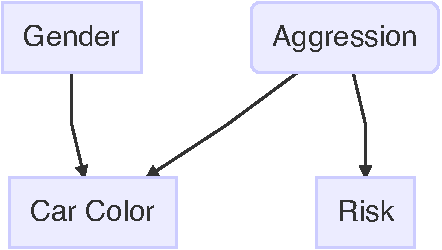
\includegraphics{ms4ds_files/figure-latex/unnamed-chunk-2-1.pdf}

In this task a car insurance company wants to predict the risk of an
insurance policy \(Y\), and the only data available to them is the car
color \(X\) and the gender \(A\) of the policy holder. The aggression
variable is an unobserved confounder. Aggression is responsible for an
observed association between \(X\) and \(Y\).

Recall the functional independence version of fairness, where we train a
function \(\hat f = \hat f(X)\) that does not take \(A\) as an input. We
can now use the causal model to understand the consequences of this type
of fairness.

Let's generate some synthetic data from this model with specific choices
for the structural equations:

\begin{Shaded}
\begin{Highlighting}[]
\NormalTok{A <-}\StringTok{ }\KeywordTok{rbinom}\NormalTok{(}\DecValTok{100}\NormalTok{, }\DecValTok{1}\NormalTok{, .}\DecValTok{5}\NormalTok{)}
\NormalTok{U <-}\StringTok{ }\KeywordTok{rnorm}\NormalTok{(}\DecValTok{100}\NormalTok{)}
\NormalTok{X <-}\StringTok{ }\NormalTok{A }\OperatorTok{+}\StringTok{ }\NormalTok{U }\OperatorTok{>}\StringTok{ }\DecValTok{1}
\NormalTok{Y <-}\StringTok{ }\NormalTok{U }\OperatorTok{>}\StringTok{ }\DecValTok{1}\OperatorTok{/}\DecValTok{2}
\NormalTok{world <-}\StringTok{ }\KeywordTok{data.frame}\NormalTok{(}\DataTypeTok{Gender =} \KeywordTok{factor}\NormalTok{(}\KeywordTok{c}\NormalTok{(}\StringTok{"Other"}\NormalTok{, }\StringTok{"Woman"}\NormalTok{)[}\KeywordTok{as.numeric}\NormalTok{(A)}\OperatorTok{+}\DecValTok{1}\NormalTok{]),}
                    \DataTypeTok{CarColor =} \KeywordTok{factor}\NormalTok{(}\KeywordTok{c}\NormalTok{(}\StringTok{"Silver"}\NormalTok{, }\StringTok{"Red"}\NormalTok{)[}\KeywordTok{as.numeric}\NormalTok{(X)}\OperatorTok{+}\DecValTok{1}\NormalTok{]),}
                    \DataTypeTok{Aggressiveness =}\NormalTok{ U,}
                    \DataTypeTok{HighRisk =}\NormalTok{ Y)}
\KeywordTok{head}\NormalTok{(world)}
\end{Highlighting}
\end{Shaded}

\begin{verbatim}
##   Gender CarColor Aggressiveness HighRisk
## 1  Other   Silver    -0.07870192    FALSE
## 2  Other   Silver     0.98316265     TRUE
## 3  Other   Silver    -0.02715656    FALSE
## 4  Woman      Red     0.48915558    FALSE
## 5  Other   Silver    -1.93444019    FALSE
## 6  Other   Silver     0.85498152     TRUE
\end{verbatim}

We can see there is no association between gender and aggressiveness:

\begin{Shaded}
\begin{Highlighting}[]
\KeywordTok{library}\NormalTok{(tidyverse)}
\KeywordTok{ggplot}\NormalTok{(world, }\KeywordTok{aes}\NormalTok{(Gender, Aggressiveness)) }\OperatorTok{+}\StringTok{ }\KeywordTok{geom_boxplot}\NormalTok{() }\OperatorTok{+}\StringTok{ }\KeywordTok{theme_minimal}\NormalTok{()}
\end{Highlighting}
\end{Shaded}

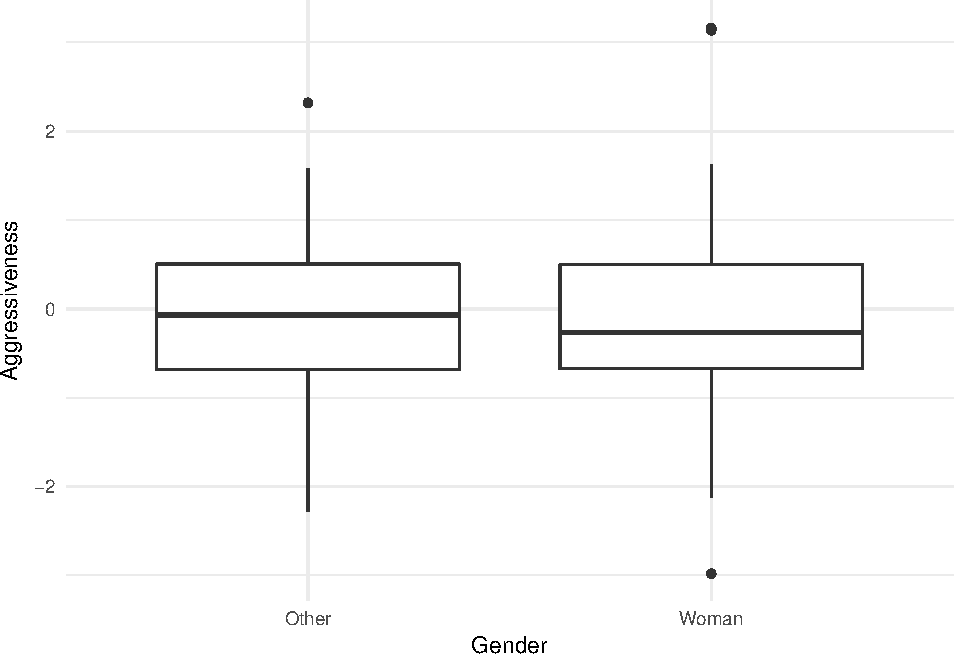
\includegraphics{ms4ds_files/figure-latex/unnamed-chunk-4-1.pdf}

But there is an association between car color and aggressiveness:

\begin{Shaded}
\begin{Highlighting}[]
\KeywordTok{ggplot}\NormalTok{(world, }\KeywordTok{aes}\NormalTok{(CarColor, Aggressiveness)) }\OperatorTok{+}\StringTok{ }\KeywordTok{geom_boxplot}\NormalTok{() }\OperatorTok{+}\StringTok{ }\KeywordTok{theme_minimal}\NormalTok{()}
\end{Highlighting}
\end{Shaded}

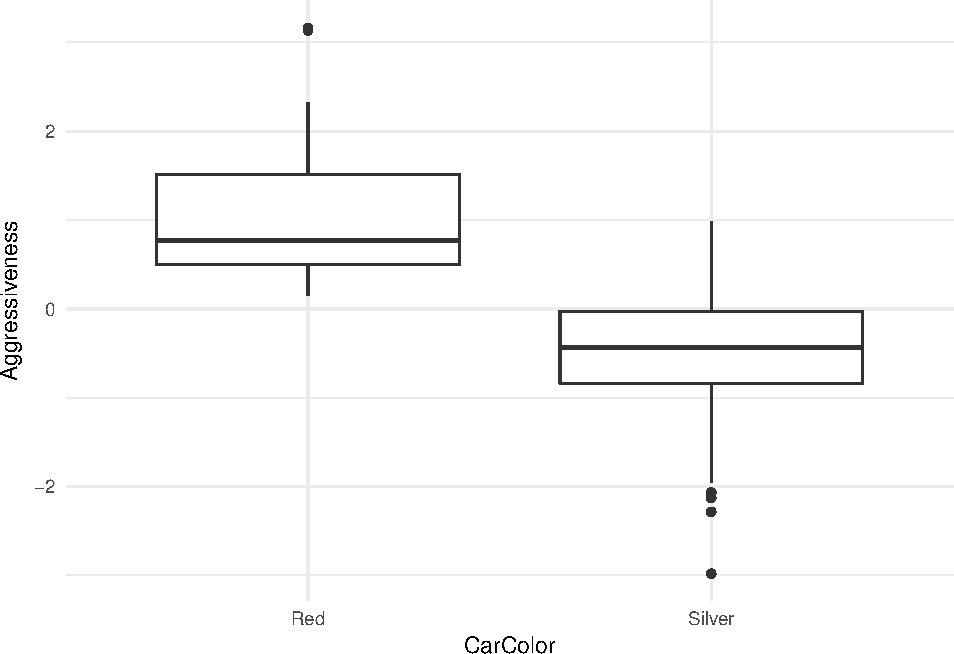
\includegraphics{ms4ds_files/figure-latex/unnamed-chunk-5-1.pdf}

Let's fit the functionally independent model, in this case using
logistic regression to predict the log odds of a binary outcome, and see
how such a model performs in predicting high risk status

\begin{Shaded}
\begin{Highlighting}[]
\KeywordTok{library}\NormalTok{(knitr)}
\NormalTok{nominal_model <-}\StringTok{ }\KeywordTok{glm}\NormalTok{(HighRisk }\OperatorTok{~}\StringTok{ }\NormalTok{CarColor, }\DataTypeTok{family =}\NormalTok{ binomial, }\DataTypeTok{data =}\NormalTok{ world)}
\NormalTok{world}\OperatorTok{$}\NormalTok{predicted <-}\StringTok{ }\KeywordTok{predict}\NormalTok{(nominal_model, }\DataTypeTok{type =} \StringTok{"response"}\NormalTok{) }\OperatorTok{>}\StringTok{ }\KeywordTok{mean}\NormalTok{(world}\OperatorTok{$}\NormalTok{HighRisk)}
\NormalTok{world }\OperatorTok\StringTok{ }\KeywordTok{group_by}\NormalTok{(Gender, HighRisk) }\OperatorTok
\StringTok{  }\KeywordTok{summarize}\NormalTok{(}\DataTypeTok{Predicted =} \KeywordTok{mean}\NormalTok{(predicted)) }\OperatorTok
\StringTok{  }\KeywordTok{kable}\NormalTok{()}
\end{Highlighting}
\end{Shaded}

\begin{verbatim}
## Warning: The `printer` argument is deprecated as of rlang 0.3.0.
## This warning is displayed once per session.
\end{verbatim}

\begin{tabular}{l|l|r}
\hline
Gender & HighRisk & Predicted\\
\hline
Other & FALSE & 0.0000000\\
\hline
Other & TRUE & 0.4666667\\
\hline
Woman & FALSE & 0.2187500\\
\hline
Woman & TRUE & 1.0000000\\
\hline
\end{tabular}

Even though there is no assocation between gender and aggression in this
world, the model misclassifies many low risk women as high risk and many
high risk men as low risk. In the US, consequences like this could
result in legal risk in some settings due to a legal theory called
\href{https://en.wikipedia.org/wiki/Disparate_impact}{disparate impact}.
But there may be a deontological argument in favor of functional
independence, including
\href{http://www.mlandthelaw.org/papers/grgic.pdf}{empirical evidence}
that people generally believe a process with functional independence is
more fair.

\subsubsection{Counterfactual fairness}\label{counterfactual-fairness}

With a mathematical causal model we can ask and answer counterfactual
questions like ``what would be the predicted risk for this person if
they were a different gender?'' The model tells us that with a different
gender, that individual might have also had a different car color,
because car color is causally influenced by gender in this world. Hence,
even though the functionally independent model does not take \(A\) as an
explicit input, it might have given a different counterfactual
prediction to a differently gendered version of the individual in
question.

We can take this further by defining fairness in terms of our
model-based counterfactuals. Let's call the learned function \(\hat f\)
\textbf{counterfactually fair} if it gives the same predictions to each
indivudal and the counterfactual version of that individual with a
different gender. This may be a very strong condition depending on the
causal model.

One drawback to this approach is that for many kinds of sensitive
attributes, like racial and gender identity, it can be difficult to
relate mathematical model-based counterfactuals to the real world. The
meaning of such counterfactuals is subject to an
\href{https://www.ncbi.nlm.nih.gov/pmc/articles/PMC4125322/}{ongoing}
\href{https://scholar.harvard.edu/files/msen/files/race_causality.pdf}{debate}
across
\href{http://www.ets.org/Media/Research/pdf/RR-03-03-Holland.pdf}{scholarly}
\href{https://papers.ssrn.com/sol3/papers.cfm?abstract_id=3050650}{disciplines}.
We now consider a brief and high level summary of this debate.

There is an argument that it only makes sense to speak of variables
being causes if those variables could be manipulated or controlled in an
experimental setting. As an example we can refer to
\href{https://www.pnas.org/content/109/41/16474.short}{randomized
experiments} evaluating biases in the evaluation of applicants to jobs
or academic programs by randomizing the names on applications. Names can
be thought of as a \textbf{proxy} for the sensitive attribute in the
sense that the person judging an application might infer a gender or
racial identity of the applicant based on the name. I consider this a
\textbf{shallow counterfactual}: what would the decision be if this
person had a different name on their application, but everything else in
their life until this point had otherwise been the same? In contrast, a
\textbf{deep counterfactual} would ask how the decision might be
different if the person had had a different name for their entire life,
implying that possibly other aspects of their application might be
different aside from their name. Proxy counterfactuals are not only
shallow, they also fail to capture what other types of things might be
different in the deep counterfactual where not only the proxy was
changed but other aspects of racial or gender identity had also been
changed. Finally, another possible position in this debate argues for
counterfactual versions of our world without the structural factors that
caused disparities in the first place. For example, how might this
person's life and the data we have for them have been different if their
ancestors had not been enslaved, subjected to racist Jim Crow laws and
redlining, and had not been deprived of generations worth of
accumulation of wealth?

\subsection{Moral luck}\label{moral-luck}

We conclude by considering another helpful concept in normative ethics
which is closely related to causation. Moral luck refers to how our
evaluation of whether someone has done good or not can depend on factors
which are outside of that person's control. The \textbf{control
principle} says that we should only judge people to the extent that the
factors we judge them on are under their control.

The control principle provides one justification for why we consider
attributes like racial or gender identity to be ``sensitive attributes''
in algorithmic fairness in the first place, and why we have laws to
protect people from discrimination on the basis of these attributes in
certain places and contexts. Such attributes are commonly understood to
be out of our individual control.

Strict application of this principle can have some dramatic and
unintuitive implications, and there are subtleties related to defining
control (or autonomy, agency, free will, etc) and deciding which things
we have control over. But the concept, combined with statistical
understanding of uncertainty and randomness, can help us arrive at
reasonable expectations and standards for moral behavior.

\subsubsection{Path-specific counterfactual
fairness}\label{path-specific-counterfactual-fairness}

Motivation for path specific fairness: some pathways may be considered
to be within our control.

Counterfactual fairness can be refined to versions where some pathways
of causation in the model are considered unfair and others are
considered fair. We can then ask for an algorithm to be counterfactually
fair when computing counterfactuals while blocking the fair pathways,
thus only requiring invariance with respect to changes that propagate
along the unfair pathways. As one possible example, consider a
predictive policing algorithm that dispatches police to patrol locations
based on historical arrest data. Due to redlining, we observe racial
disparities in neighborhood demographics, and historically there were
higher rates of policing in majority-minority neighborhoods and
therefore higher rates of arrests. We summarize this hypothetical world
in the graph below:

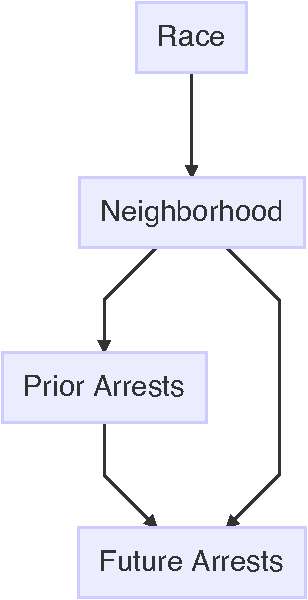
\includegraphics{ms4ds_files/figure-latex/unnamed-chunk-7-1.pdf}

One possible application of path-specific fairness in this graph is as
follows. We wish to avoid predicting higher rates of arrests on the
basis of race, and since we know that race has historically influenced
which neighborhood someone lives in we understand that we cannot simply
predict using the neighborhood variable without potentially having a
disparate impact. However, someone may argue that the pathway
\(\text{Prior Arrests} \to \text{Future Arrests}\) should be considered
fair based on the assumption that avoiding behavior that might result in
arrest is within a person's control. Someone else may argue that this
pathway is still unfair because being arrested is still at least
partially a matter of luck. It's not in an individual's control to
decide what level of policing their neighborhood is subjected to, and
it's unfair that people behaving in ways that could result in arrest in
other neighborhoods are not arrested simply because they were not
caught.

\section{Conclusion}\label{conclusion}

Taken together, the growing body of empirical research that can help us
understand real world causes, mathematical causal models, definitions of
fairness using counterfactuals and path-specific counterfactuals, and a
variety of normative ethical frameworks provide us with a powerful set
of tools for understanding the ethical implications of a given data
science task. There are still challenges, especially regarding modeling
choices which will almost always rely on some assumptions that are not
testable. In some scenarios we may not be able to arrive at a consensus
on one adequate causal model or one set of choices regarding which
pathways in a given model are fair. But we can at least have a common
framework in which to have those discussions, the framework directs our
attention toward causal relationships, and it allows/forces us to make
our assumptions explicit and transparent. Even in settings when we
cannot reach consensus, if we can arrive at a small enough set of models
which are not too mutually contradictory, we can use
\href{https://papers.nips.cc/paper/7220-when-worlds-collide-integrating-different-counterfactual-assumptions-in-fairness}{algorithmic
methods} to approximately satisfy counterfactual fairness simultaneously
for each model.

Finally, even if we are not fully committed to causal approaches to
fairness or ethics in the sense that we will derive our actual actions
from them, we can still use them as thought experiments and diagnostic
methods. They can help us to understand the limitations of other
methods, identify ethically sensitive aspects of the data science task,
and even find ways to intervene or change the task formulation.

\section{Additional reading}\label{additional-reading}

General data science ethics

\begin{itemize}
\tightlist
\item
  \textbf{Statement}:
  \href{https://www.amstat.org/ASA/Your-Career/Ethical-Guidelines-for-Statistical-Practice.aspx}{Ethical
  Guidelines for Statistical Practice} by the American Statistical
  Association
\item
  Statement: \href{https://www.acm.org/code-of-ethics}{Code of Ethics
  and Professional Conduct} by the Association for Computing Machinery
\item
  Statement:
  \href{https://www.gov.uk/government/publications/data-ethics-framework/data-ethics-framework}{Data
  Ethics Framework} by the UK Government
\item
  Short book:
  \href{https://resources.oreilly.com/examples/0636920203964}{Ethics and
  Data Science} by Mike Loukides, Hilary Mason, and DJ Patil (Patil was
  Chief Data Scientist during the Obama administration)
\item
  Book: \href{https://bookbook.pubpub.org/data-feminism}{Data Feminism}
  by Catherine D'Ignazio and Lauren Klein
\item
  Book:
  \href{https://press.anu.edu.au/publications/series/caepr/indigenous-data-sovereignty}{Indigenous
  Data Sovereignty} edited by Tahu Kukutai and John Taylor
\item
  \textbf{Book}: \href{https://www.bitbybitbook.com/en/ethics/}{Bit by
  Bit (Ethics Chapter)} by Matthew Salganik
\item
  Case studies:
  \href{https://aiethics.princeton.edu/case-studies/case-study-pdfs/}{Collection
  of fictional case studies} by the Princeton Dialogues on AI and Ethics
\end{itemize}

Fairness and causal models

\begin{itemize}
\tightlist
\item
  Articles:
  \href{https://phenomenalworld.org/digital-ethics/disparate-causes-i}{Disparate}
  \href{https://phenomenalworld.org/digital-ethics/disparate-causes-pt-ii}{Causes}
  by Lily Hu
\item
  Paper: \href{https://arxiv.org/abs/1805.05859}{Causal Reasoning for
  Algorithmic Fairness} by Joshua Loftus, Chris Russell, Matt Kusner,
  and Ricardo Silva
\end{itemize}

Stanford Encyclopedia of Philosophy

\begin{itemize}
\tightlist
\item
  \href{https://plato.stanford.edu/archives/spr2019/entries/informed-consent/}{Informed
  Consent} by Nir Eyal
\item
  \href{https://plato.stanford.edu/archives/sum2018/entries/ethics-computer/}{Computer
  and Information Ethics} by Terrell Bynum
\item
  \href{https://plato.stanford.edu/entries/ethics-social-networking/}{Social
  Networking and Ethics} by Shannon Vallor
\item
  \href{https://plato.stanford.edu/archives/fall2016/entries/ethics-search/}{Search
  Engines and Ethics} by Herman Tavani
\item
  \href{https://plato.stanford.edu/archives/fall2017/entries/ethics-business/}{Business
  Ethics} by Jeffrey Moriarty
\end{itemize}

\chapter{Foundations of inference}\label{foundations-of-inference}

\section{Philosophy of statistics}\label{philosophy-of-statistics}

In general it is a good habit to (re-)examine one's beliefs, but there
are also good reasons to study philosophy specific to statistics and
data science.

What is the meaning of probability? Kolmogorov's axioms describe a kind
of mathematical model, but what relation do such models have to the real
world, if any? The same set of axioms can be used (and fruitfully!) to
describe:

\begin{itemize}
\tightlist
\item
  Hypothetical \textbf{properties of the physical world}, as in most
  interpretations of quantum physics, or the ``\textbf{propensity}'' of
  a dice to land on a particular side
\item
  \textbf{Degrees of subjective belief}, or confidence, that a given
  individual has about states of the world
\item
  \textbf{Logical rules} governing quantitative relationships between
  hypotheses and evidence
\end{itemize}

\subsection{Additional reading}\label{additional-reading-1}

\url{https://en.wikipedia.org/wiki/Probability_interpretations}
\url{https://plato.stanford.edu/entries/probability-interpret/}
\url{https://en.wikipedia.org/wiki/Foundations_of_statistics}
\url{https://en.wikipedia.org/wiki/Philosophy_of_science}

\section{Hypothesis testing
background}\label{hypothesis-testing-background}

\subsection{Hypothesis formulation: a neglected topic in data science
education?}\label{hypothesis-formulation-a-neglected-topic-in-data-science-education}

\section{Causality}\label{causality}

\chapter{Large scale testing}\label{large-scale-testing}

\section{Multiple testing}\label{multiple-testing}

\subsection{Family-wise error rate}\label{family-wise-error-rate}

\subsection{Special cases: groups and
hierarchy}\label{special-cases-groups-and-hierarchy}

\section{Selective inference}\label{selective-inference}

\subsection{False discovery rate}\label{false-discovery-rate}

\subsection{Special cases: groups and
hierarchy}\label{special-cases-groups-and-hierarchy-1}

\section{Empirical Bayes approaches}\label{empirical-bayes-approaches}

\chapter{Causal inference}\label{causal-inference}

\section{A variety of treatment
effects}\label{a-variety-of-treatment-effects}

\section{Directed acyclic graphs and structural equation
models}\label{directed-acyclic-graphs-and-structural-equation-models}

\subsection{Common problems?}\label{common-problems}

\begin{itemize}
\tightlist
\item
  Selection bias
\item
  Conditioning on colliders
\end{itemize}

\chapter{Foundations of regression}\label{foundations-of-regression}

\section{Philosophy of regression
models}\label{philosophy-of-regression-models}

\begin{itemize}
\tightlist
\item
  Why assume errors are Gaussian?
\item
  False hope of causality
\end{itemize}

\section{Linear regression}\label{linear-regression}

\section{Generalized linear models and exponential
families}\label{generalized-linear-models-and-exponential-families}

\section{Inference in regression
models}\label{inference-in-regression-models}

\section{Model diagnostics}\label{model-diagnostics}

\chapter{Machine learning and high dimensional
regression}\label{machine-learning-and-high-dimensional-regression}

Expanding our set of regression-like tools

\section{Lasso and penalized
regression}\label{lasso-and-penalized-regression}

\section{Generalized additive models}\label{generalized-additive-models}

\section{Trees, forests, boosting}\label{trees-forests-boosting}

\chapter{Selective inference}\label{selective-inference-1}

\section{Conditional approach}\label{conditional-approach}

\section{Debiasing approaches}\label{debiasing-approaches}

\chapter{Machine learning for causal
inference}\label{machine-learning-for-causal-inference}

\section{Double machine learning}\label{double-machine-learning}

\section{Weight-based approaches}\label{weight-based-approaches}

\bibliography{book.bib,packages.bib}


\end{document}
